\documentclass[usenames,dvipsnames]{beamer}
% \documentclass[usenames,dvipsnames,handout]{beamer}

\usetheme{AnnArbor}
%\usetheme{Boadilla}
\usecolortheme{beaver}
\usecolortheme{dolphin}
% \usecolortheme{orchid}
% \usecolortheme{rose}


\usepackage{fourier}
\usepackage{faktor}
\usepackage{amssymb}
\usepackage{amsmath}
\usepackage{amsthm}
\usepackage{stmaryrd}
\usepackage{hyperref}
\usepackage[all]{xy}
\usepackage[final]{pdfpages}
\usepackage{tikz}
    \usetikzlibrary{mindmap,shadows,shapes.geometric,shapes.misc,positioning}
\usepackage{xcolor}
\usepackage{multirow}
\usepackage{pbox}
\newcommand{\pboxc}[2]{\pbox{#1}{\relax\ifvmode\centering\fi#2}}
\usepackage{cellspace}
\setlength{\cellspacetoplimit}{2pt}
\setlength{\cellspacebottomlimit}{2pt}

%\newcommand{\downmapsto}{\rotatebox[origin=c]{-90}{$\large\mapsto$}\mkern2mu} %MnSymbol doesn't work well with beamer
\usepackage{array}
\newcolumntype{P}[1]{>{\centering\arraybackslash}p{#1}}
\newcolumntype{M}[1]{>{\centering\arraybackslash}m{#1}}

\def\Q{\mathbb{Q}}
\def\Z{\mathbb{Z}}
\def\C{\mathbb{C}}
\def\R{\mathbb{R}}
\def\F{\mathbb{F}}

\DeclareMathOperator{\Mat}{Mat}
\DeclareMathOperator{\Char}{char}
%\renewcommand{\char}{char} problems with xymatrix
\DeclareMathOperator{\rk}{Rank}
\DeclareMathOperator{\Frob}{Frob}
\DeclareMathOperator{\bICM}{\overline{\ICM}}
\DeclareMathOperator{\ICM}{ICM}
\DeclareMathOperator{\Cl}{Cl}
\DeclareMathOperator{\Wk}{\cW}
\DeclareMathOperator{\bWk}{\overline{\Wk}}
\DeclareMathOperator{\Pic}{Pic}
\DeclareMathOperator{\Aut}{Aut}
\DeclareMathOperator{\Hom}{Hom}
\DeclareMathOperator{\End}{End}
\DeclareMathOperator{\mSpec}{mSpec}
\DeclareMathOperator{\GL}{GL}
\DeclareMathOperator{\Tr}{Tr}



\newcommand{\cB}{{\mathcal B}}
\newcommand{\cC}{{\mathcal C}}
\newcommand{\cI}{{\mathcal I}}
\newcommand{\cM}{{\mathcal M}}
\newcommand{\cO}{{\mathcal O}}
\newcommand{\cQ}{{\mathcal Q}}
\newcommand{\cR}{{\mathcal R}}
\newcommand{\cW}{{\mathcal W}}

\newcommand{\vphi}{\varphi}

\newcommand{\p}{{\mathfrak p}}
\newcommand{\frf}{{\mathfrak f}}

\newcommand{\set}[1]{\left\lbrace#1\right\rbrace }
\newcommand{\Span}[1]{\left<#1\right>}

\newcommand{\isoclass}[1]{[#1]}
\newcommand{\wkclass}[1]{\{ #1 \}}

\newcommand{\red}[1]{\textcolor{red}{#1}}
\newcommand{\blue}[1]{\textcolor{blue}{#1}}
\newcommand{\green}[1]{\textcolor{ForestGreen}{#1}}

\usepackage{eurosym}

\newtheorem{df}{Definition}[section]
\newtheorem{remark}[df]{Remark}
\newtheorem{proposition}[df]{Proposition}

%AUTHOR DETAILS
%%%%%%%%%%%%%%%%%%%%%%%%%%%%%%%%%%%%%%%%%%%%%%%%
\title[CPJ - Université Côte d'Azur]{Chair de Professeur Junior - Université Côte d'Azur}
\subtitle{}
\author[Stefano Marseglia]{Stefano Marseglia}
% \institute[]{Utrecht University}
\date[21 June 2022 ]{}

\begin{document}

\begin{frame}
\titlepage
{ \vspace{-1.5cm}\footnotesize
Short resum\'e:
\begin{itemize}
     \item 06/2008 - 07/2011 : Bachelor degree, University of Turin.
     \item 09/2011 - 07/2013 : ALGANT Master, double degree, Padova-Leiden.
     \item 08/2013 - 07/2018 : PhD, Stockholm University, w/ Jonas Bergstr\"om.
     \item 09/2018 - 12/2018 : Postdoc, Max Planck Institute, Bonn.
     \item 01/2019 - 12/2020 : Postdoc, Utrecht University, w/ Carel Faber.
     \item 01/2021 - 12/2023 : Veni Postdoc, Utrecht University.
\end{itemize}
Major grants:
\begin{itemize}
     \item Veni grant, Dutch research council, 250.000\euro.
     \item to go to MIT, K\&A Wallenbergs (declined in favour of the Veni), 130.000\$.
\end{itemize}
}
\end{frame}

\begin{frame}
     \begin{center}
          {\Large
          Overview of my research}
     \end{center}
\end{frame}
\begin{frame}
     \begin{center}
     \begin{tikzpicture}[
          % squarenodered/.style={rectangle, draw=red!60, fill=red!5, very thick, minimum size=5mm},
          % squarenodeblue/.style={rectangle, draw=blue!60, fill=blue!5, very thick, minimum size=5mm},
          squarenodepurple/.style={rectangle, draw=Black!60, fill=Black!5, very thick, minimum size=5mm},
          % CAlg/.style={rectangle},
          ]
          \onslide<1->{
               \begin{scope}[blend group=darken]
                    \filldraw[color=red!60, fill=red!30] (-2,0) ellipse (3cm and 2cm);
                    \filldraw[color=blue!60, fill=blue!30] (2,0) ellipse (3cm and 2cm);
                    \onslide<4->{\filldraw[color=Orange!60, fill=Yellow!30] (0,-2) ellipse (3cm and 2cm);}
               \end{scope}
               \node (AGset) at (-3,0)
                    {\parbox[c]{4em}{\Large Algebraic\\ Geometry}};
               \node (NTset) at (3,0)
                    {\parbox[c]{4em}{\Large Number\\ Theory}};
          }
          \onslide<4->{
               \node (CAlg) at (-0.5,-2.8)
                    {\parbox[c]{4em}{\centering \Large Commutative \\ Algebra}};   
          }
          \onslide<2->{
                 \node[squarenodepurple] (AV) at (-0.5,2.8)    
                      {\parbox[c]{7.5em}{\centering Abelian Varieties: \\ add two points}};
                 \draw [-,Black, very thick] (AV.south) .. controls (-0.5,1) ..  (0,0);
          }
          \onslide<3-4>{
                  \node[right=1cm of AV, anchor=west, yshift=-0.5cm] (Abel)
                             {\parbox{3.5cm}{\centering Niels Abel \footnotesize(1802-1829)\\
                                              \includegraphics[width=3.5cm]{fig_abel.jpeg}
                             }};
                  \draw [dotted,black,very thick] (Abel) to [out=180,in=0] (AV);
          }
          \onslide<5->{
               \filldraw[color=Black!60, fill=Black!30] (0,0) circle (2cm);
               \node (Comp) at (-0.5,0)
                    {\parbox[c]{4em}{\centering \Large Computations \\ Algorithms}};
               }
          \end{tikzpicture}      
     \end{center}
\end{frame}

\begin{frame}{ Abelian varieties: an example }
\vspace{-0.5cm}
\begin{center}
	\begin{columns}
		\begin{column}{0.4\textwidth}
			\onslide<1->{Abelian varieties of dim.~$1$\\
                            are called {\bf elliptic curves}.\\
                            Eg: over $\R$, $\red{y^2 = x^3 -x +1}$
                            \vspace{1em}}
               % \vpsace{1em}
			\onslide<2->{We can add points:\\
                            $P,Q$ {\Large \blue{$\leadsto$}} $P\oplus Q$
                            \vspace{1em}\\
                            }
               \onslide<3->{Equations are impractical in $\dim \geq 2$.\\
                            We need a better way to represent them...}             
		\end{column}
		\begin{column}{0.5\textwidth}
			\tikz{
			    \onslide<1->{
				\draw [help lines] (-2,-2.24) grid (1.8,2.24);
				\draw [->] (-2-0.2,0) -- (1.8+0.2,0) node[right] {$x$}; 
				\draw [->] (0,-2.24-0.2) -- (0,2.24+0.2) node[left] {$y$}; 
				\draw [red, thick, domain=-1.32471795724474602596090885448:1.8, samples=100]
				 plot (\x, {sqrt(\x*\x*\x -\x +1)});
				\draw [red, thick, domain=-1.32471795724474602596090885448:1.8, samples=100]
				 plot (\x, -{sqrt(\x*\x*\x -\x +1)});
				}
				\onslide<2->{
				\draw [blue, thick, domain=-2:1.8, samples=100] plot (\x, {0.7*\x +0.5 });
				\draw [blue, thick, dashed] (1.3407,2.24) -- (1.3407,-2.24);
				\draw (-1.2858-0.2,-0.7*1.2858+0.5+0.1) node {$P$};
				\draw (0.43506,0.7*0.43506+0.5 +0.3) node {$Q$};
				\draw (1.3407+0.5,-0.7*1.3407-0.5) node {$P\oplus Q$};
				}
			}
		\end{column}
	\end{columns}
\end{center}
\end{frame}

\begin{frame}{ }
\setbeamercovered{
  again covered={\opaqueness<1->{20}}
}
\begin{tikzpicture}
    [
    every annotation/.style = {draw,fill = white},
    mainchar/.style={circle, draw=red!60, fill=red!5, very thick, minimum size=5mm},
    problem/.style={regular polygon, regular polygon sides=3,
                     draw=ForestGreen!60, fill=green!5, very thick, minimum size=35mm},
    frobenius/.style={rectangle, draw=blue!60, fill=blue!5, very thick, minimum size=5mm},
    HondaTate/.style={rectangle, ,rounded corners=1ex, draw=blue!60, fill=blue!5, very thick, minimum size=5mm},
    goals/.style={draw=Plum!60, fill=Plum!5, very thick}, 
    goals_spec/.style={rectangle, draw=Plum!60, fill=Plum!5, very thick, minimum size=5mm},       
    applications/.style={rectangle, rounded corners=1ex, draw=YellowOrange!60, fill=YellowOrange!5, very thick, minimum size=5mm},
    applications_spec/.style={rectangle, draw=YellowOrange!60, fill=YellowOrange!5, very thick, minimum size=5mm},  
    extra/.style={ellipse, draw=Black!100, fill=Black!5, very thick, minimum size=5mm},  
    ]
    \onslide<1-7,9-12,14,16->{
    \node[mainchar] (AbVarFq) at (-3,0) {
                                          \parbox{1.5cm}{\centering \bf
		                                   Abelian\\
		                                   Varieties\\
		                                   over $\F_{p^k}$}
		                                 };
    }

    \onslide<2-7,9-12,14,16->{
    \node[problem] (hard) at (-3,4) {};
    \node at (-3,4) {
		                \parbox{3.65cm}{\footnotesize\centering
		                can't use\\
		                derivatives,\\
		                differentiation,\\
		                ... }
                    };
    \draw[-,draw=ForestGreen!60, very thick]
         (AbVarFq) to [out=135,in=-135]
         node[inner sep=.05cm,fill=white] {\footnotesize hard!}
         (hard);
    }

    \onslide<3-7,9-12,14,16->{
    \node[frobenius] (frobenius) at (-1,2) {extra structure};
    \draw[-,draw=blue!60, very thick] (AbVarFq) to [out=45,in=-155] (frobenius);
    }

    \onslide+<4>{
     \node[extra, right=0.5cm of frobenius, anchor=west] (frob_extra) 
               {
                    \parbox{2cm}{\centering Frobenius $x\mapsto x^p$}
               };
               \draw[-,draw=Black!100, very thick] (frob_extra) to [out=180,in=0] (frobenius);
     }

    \onslide<5-12,14,16->{
    \node[HondaTate] (HondaTate) at (.5,5) 
            {\pbox{\textwidth}{
	          isogeny classification:\\
	          \footnotesize
		     $\bullet$ Honda-Tate~('68-'71)\\
               $\bullet$ ``coarse''
			}};
    }
    \onslide<5-7,9-12,14,16->{
          \draw[->,draw=blue!60, very thick] 
          (frobenius) to [out=35,in=-90] 
          node[inner sep=.05cm,fill=white] {\footnotesize exploit:}
          (HondaTate);
     }
    \onslide<6-7,9-12,14,16->{
     \node[goals, right=3.0cm of HondaTate,ellipse, minimum height=10mm, minimum width=19.5mm] (goals) { };
     \node[right=2.95cm of HondaTate] {\bf Objectives};
     \draw[->,draw=blue!60, very thick] 
          (HondaTate) to 
          node[above, inner sep=.05cm] 
          {\pbox{2.5cm}{\footnotesize starting point:\\ fix an isogeny class}}
          (goals);
    }
    \onslide<7-12,14,16->{
     \node[goals_spec, below=-0.1cm of goals, anchor=north east, xshift=2mm] 
          (isom) {
                    \pbox{\textwidth}{
                         ``finer'' classification:\\
                         up to isomorphism
                         \vspace{-0.3em}\\
                         {\tiny $\star$ Bergstr\"om SU, Karemaker UU}
                    }
                    };
    }
    \onslide+<8>{
          \node[extra, right=-0.5cm of HondaTate, anchor=south west, yshift=0.2cm] (isog_extra) 
                    {
                         \parbox{4cm}{\centering isogeny : \\ surjective + finite kernel}
                    };
          \node[extra, left=0.1cm of isom, anchor=east, yshift=-0.5cm] (isom_extra) 
                    {
                         \parbox{4cm}{\centering isomorphism : \\ surjective + trivial kernel}
                    };
                    \draw[-,draw=Black!100, very thick] (isom_extra) to [out=-15,in=-90] (isom);
                    \draw[-,draw=Black!100, very thick] (isog_extra) to [out=155,in=90] (HondaTate);
     }


    \onslide<9-12,14,16->{
    \node[goals_spec, below=0cm of isom, anchor=north, xshift=-0.5cm] 
         (pols)
          {polarizations
               % \pbox{\textwidth}{polarizations\vspace{-0.3em}\\
               % {\tiny $\square$ IMRN Bergstr\"om SU - Karemaker UU}}
          };
    }
    \onslide<10-12,14,16->{
          \node[goals_spec, below=0.5cm of pols, anchor=north west, xshift=0.1cm]
               (moduli) {moduli space};
          \draw[->,draw=Plum!60, very thick] (isom) to [out=0,in=60] (moduli);
          \draw[->,draw=Plum!60, very thick] (pols) to [out=0,in=80] (moduli);
    }
    \onslide<11-12,14,16->{
    \node[goals_spec, below=0.5 cm of pols, anchor=north east]
         (compute) {compute data};

    \draw[->,draw=Plum!60, very thick] (isom) to [out=180,in=140] (compute);
    \draw[->,draw=Plum!60, very thick] (pols) to [out=180,in=120] (compute);
    }
    \onslide<12,14,16->{          
    \node[applications] (applications) at (3,0) { \bf Applications};
    }
    \onslide<12-14,16->{    
    \node[applications_spec, left=0cm of applications, anchor=east]
         (lmfdb) 
         {
               \pbox{\textwidth}{publish online\vspace{-0.3em}\\
               {\tiny $\star$ Costa, Roe MIT, et.~al.}}

          };
    }
    \onslide<12,14,16->{ 
    \draw[->,draw=Plum!60, very thick] (compute) to [out=270,in=120] (applications);
    }
    \onslide+<13>{    
    \node[right=0.1cm of lmfdb, anchor=west] 
            {
            {%
				\setlength{\fboxsep}{0pt}%
				\setlength{\fboxrule}{1pt}%
				\fbox{\includegraphics[width=5cm]{fig_lmfdb_screenshot.png}}
            }
            };
    }
    \onslide<14,15->{
    \node[applications_spec, right=1 cm of applications, anchor=north, yshift=-0.5cm]
         (crypto) {\pbox{\textwidth}{
                         isogeny graphs\vspace{-0.3em}\\
                         {\tiny $\star$ Arpin LU, Springer HI}
                    }};
    }
    \onslide<14,16->{
    \draw[->,draw=YellowOrange!60, very thick] (crypto) to [out=180,in=-75] (applications);
    }
    \onslide+<15>{
    \node[left=0.2cm of crypto, anchor=south east]
               {
               {%
				\setlength{\fboxsep}{0pt}%
				\setlength{\fboxrule}{1pt}%
				\fbox{\includegraphics[width=6cm]{fig_isog_graph.jpg}}
               }
               };
    }
    \onslide<16>{
    \node[applications_spec, left=1 cm of applications, anchor=north, yshift=-0.7cm]
         (crypto) {
               \pbox{\textwidth}{correcting codes\vspace{-0.3em}\\
               {\tiny $\star$ Berardini CPJ at IMB}
               }};
    \draw[->,draw=YellowOrange!60, very thick] (crypto) to [out=0,in=-105] (applications);
    }     
\end{tikzpicture}	
\end{frame}


\begin{frame}{Some highlight of my research output}
     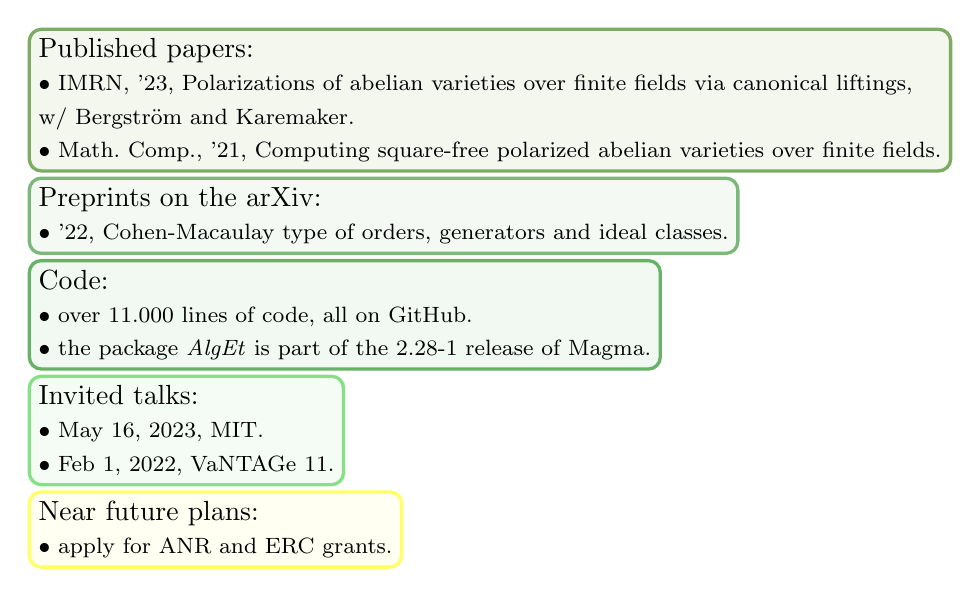
\begin{tikzpicture}
          [
          objective/.style = {fill = white},
          papers/.style={rectangle, rounded corners=1ex, draw=OliveGreen!60, fill=OliveGreen!5, very thick, minimum size=5mm},
          preprint/.style={rectangle, rounded corners=1ex, draw=ForestGreen!60, fill=ForestGreen!5, very thick, minimum size=5mm},
          code/.style={rectangle, rounded corners=1ex, draw=Green!60, fill=Green!5, very thick, minimum size=5mm},
          conf/.style={rectangle, rounded corners=1ex, draw=LimeGreen!60, fill=LimeGreen!5, very thick, minimum size=5mm},
          future/.style={rectangle, rounded corners=1ex, draw=Yellow!60, fill=Yellow!5, very thick, minimum size=5mm},
          ]
          \onslide<2->{
               \node[papers] (papers) at (0,0) {
                         \pbox{\textwidth}{
                              Published papers:\\
                              {\footnotesize $\bullet$ IMRN, '23,
                              Polarizations of abelian varieties over finite fields via canonical liftings,}\\
                              {\footnotesize w/ Bergström and Karemaker.}\\
                              {\footnotesize $\bullet$ Math.~Comp., '21,
                              Computing square-free polarized abelian varieties over finite fields.}
                         }
                    };
          }
          \onslide<3->{
               \node[preprint, below=0.05cm of papers.south west, anchor=north west ] (preprint) {
                         \pbox{\textwidth}{
                              Preprints on the arXiv:\\
                              {\footnotesize $\bullet$ '22,
                              Cohen-Macaulay type of orders, generators and ideal classes.}
                         }
                    };
          }
          \onslide<4->{
               \node[code, below=0.05cm of preprint.south west, anchor=north west ] (code) {
                         \pbox{\textwidth}{
                              Code:\\
                              {\footnotesize $\bullet$ over 11.000 lines of code, all on GitHub.}\\
                              {\footnotesize $\bullet$ the package \emph{AlgEt} is part of the $2.28$-$1$ release of Magma.}
                         }
                    };
          }
          \onslide<5->{
               \node[conf, below=0.05cm of code.south west, anchor=north west ] (conf) {
                         \pbox{\textwidth}{
                              Invited talks:\\
                              {\footnotesize $\bullet$ May 16, 2023, MIT.}\\
                              {\footnotesize $\bullet$ Feb 1, 2022, VaNTAGe 11.}
                         }
                    };
          }
          \onslide<6->{
               \node[future, below=0.05cm of conf.south west, anchor=north west ] (future) {
                         \pbox{\textwidth}{
                              Near future plans:\\
                              {\footnotesize $\bullet$ apply for ANR and ERC grants.}
                         }
                    };
          }
     \end{tikzpicture}	
\end{frame}

\begin{frame}
     \begin{center}
          {\Large
          Integration in the local mathematical community.
          }
     \end{center}
\end{frame}

\begin{frame}{}\
     \begin{tikzpicture}
          [
               every annotation/.style = {draw,fill = white},
               abvar/.style={circle, draw=red!60, fill=red!5, very thick, minimum size=5mm},
               abvarbox/.style={rectangle, rounded corners=1ex, draw=red!60, fill=red!5, very thick, minimum size=5mm},
               delmod/.style={circle, draw=ForestGreen!60, fill=ForestGreen!5, very thick, minimum size=5mm},
               delmodbox/.style={rectangle, rounded corners=1ex, draw=ForestGreen!60, fill=ForestGreen!5, very thick, minimum size=5mm},
               mats/.style={circle, draw=blue!60, fill=blue!5, very thick, minimum size=5mm},
               matbox/.style={rectangle, rounded corners=1ex, draw=blue!60, fill=blue!5, very thick, minimum size=5mm},
               ring/.style={rectangle, rounded corners=1ex, draw=black!60, fill=black!5, very thick, minimum size=5mm},
               coll/.style={rectangle, rounded corners=1ex, draw=YellowOrange!60, fill=YellowOrange!5, very thick, minimum size=5mm},
          ]
          \onslide<1-7>{
               \node[abvar] (abvar) at (3,0) {
                                             \parbox{1.5cm}{\centering \bf
                                                  Abelian\\
                                                  Varieties\\
                                                  over $\F_{p^k}$}
                                             };
          }
          \onslide+<2-3>{    
               \node[abvarbox, left=1cm of abvar] (abvarbox)
               {
                    \pbox{\textwidth}{{\bf Possible collaborations:}\\
                                        - Christophe Ritzenthaler CIMPA, (Rennes)\\
                                        - his PhD student Thomas Bouchet\\
                                        - group in Luminy (Kohel, Anni, Aubry, ...)\\
                                        \onslide+<3>{- H\"oring [K3, Prym] UCA\\
                                             - Simpson [moduli] UCA\\
                                             - Beauville UCA
                                        }
                    }
               };
               \draw[->,draw=black,thick] (abvar) to (abvarbox); 
          }
          \onslide<4->{
          \node[delmod] (delmod) at (3,5) {
                                             \parbox{1.5cm}{\centering \bf
                                             Deligne modules}
                              };
          }
          \onslide<4-7>{
               \draw[-,draw=ForestGreen!60, very thick]
               (abvar) to [out=90,in=-90]
               node[inner sep=.05cm,fill=white] {\footnotesize how to represent them?}
               (delmod);
          }
          \onslide<5->{    
               \node[delmodbox, left=1cm of delmod] (delmodbox) {
                    \pbox{\textwidth}{
                         fin.~gen.~torsionfree\\
                         modules over $R=\frac{\Z[x,y]}{(h(x,y),xy-p^k)}$
                    }
               };
          \draw[->,draw=black,thick] (delmod) to (delmodbox); 
          }
          \onslide<6->{
               \node[mats] (mats) at (-4,0) {
                    \pbox{\textwidth}{\bf
                         $\GL_n(\Z)$-conj.\\
                         classes of\\
                         $\Z$-matrices}
                    };
                    \draw[-,draw=black!60, very thick, dotted]
                    (delmod) to [out=-135,in=45]
                    % node[inner sep=.05cm,fill=white] {\footnotesize how to represent them?}
                    (mats);     
          }
          \onslide<6-7>{
               \draw[-,draw=black!60, very thick, dotted]
               (abvar) to 
               % node[inner sep=.05cm,fill=white] {\footnotesize how to represent them?}
               (mats);
          }
          \onslide<7->{    
               \node[matbox, above=0.3cm of mats] (matbox) {
                    \pbox{\textwidth}{
                         fin.~gen.~torsionfree\\
                         modules over $R=\frac{\Z[x]}{(h(x))}$
                    }
               };
               \draw[->,draw=black,thick] (mats) to (matbox); 
          }
          \onslide<8->{    
               \node[ring] (ring) at (2,3) {
                    \pbox{\textwidth}{
                         $R$ is often singular! Need tools from \\
                         commutative algebra\\ 
                         {\footnotesize (Gorenstein, Cohen-Macaulay type,...) }
                    }
               };
               \draw[->,draw=black,very thick] (ring) to (delmodbox); 
               \draw[->,draw=black,very thick] (ring) to (matbox); 
          }
          \onslide<9->{    
               \node[coll, below=0.5cm of ring] (coll) {
                    \pbox{\textwidth}{ {\bf Possible collaborations}\\
                         Laurent Busé INRIA, Aromath\\
                         Bernard Mourrain INRIA, Aromath
                    }
               };
               \draw[<->,draw=black,very thick] (ring) to (coll); 
          }
\end{tikzpicture}	
\end{frame}

\begin{frame}
     \begin{center}
          {\Large
          Teaching and mentoring
          }
     \end{center}
\end{frame}

\begin{frame}{Highlights of my teaching experience}
     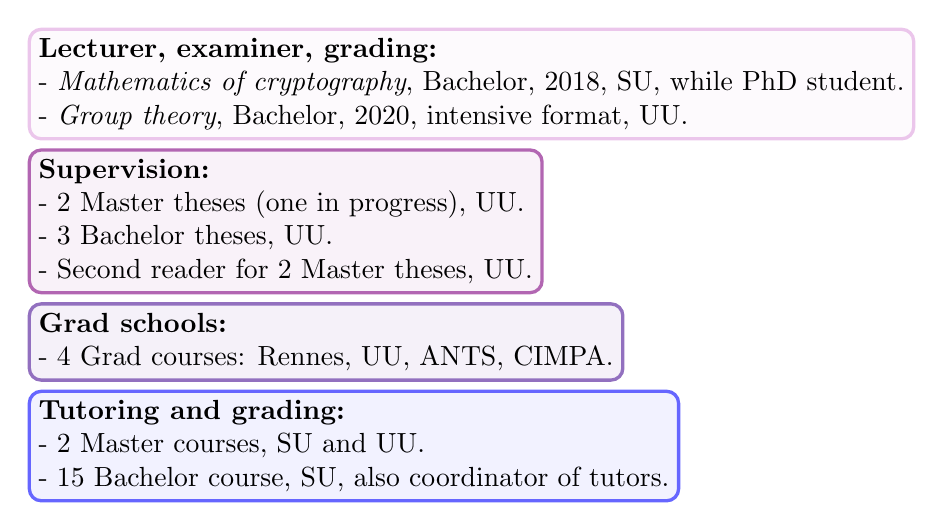
\begin{tikzpicture}
          [
          objective/.style = {fill = white},
          lect/.style={rectangle, rounded corners=1ex, draw=Plum!60, fill=Plum!5, very thick, minimum size=5mm},
          superv/.style={rectangle, rounded corners=1ex, draw=Purple!60, fill=Purple!5, very thick, minimum size=5mm},
          grad/.style={rectangle, rounded corners=1ex, draw=RoyalPurple!60, fill=RoyalPurple!5, very thick, minimum size=5mm},
          tutor/.style={rectangle, rounded corners=1ex, draw=blue!60, fill=blue!5, very thick, minimum size=5mm},
          ]
          \onslide<2->{
               \node[lect] (lect) at (0,0) {
                         \pbox{\textwidth}{
                              {\bf Lecturer, examiner, grading:}\\
                              - \emph{Mathematics of cryptography}, Bachelor, 2018, SU, while PhD student.\\
                              - \emph{Group theory}, Bachelor, 2020, intensive format, UU.
                         }
                    };
          }
          \onslide<3->{
               \node[superv, below=0.1cm of lect.south west, anchor=north west ] (superv) {
                         \pbox{\textwidth}{
                              {\bf Supervision:}\\
                              - 2 Master theses (one in progress), UU.\\
                              - 3 Bachelor theses, UU.\\
                              - Second reader for 2 Master theses, UU.
                              % - Group supervisor for several courses, SU and UU.
                         }
                    };
          }
          \onslide<4->{
               \node[grad, below=0.1cm of superv.south west, anchor=north west ] (grad) {
                         \pbox{\textwidth}{
                              {\bf Grad schools:}\\
                              - 4 Grad courses: Rennes, UU, ANTS, CIMPA.
                         }
                    };
          }
          \onslide<5->{
               \node[tutor, below=0.1cm of grad.south west, anchor=north west ] (tutor) {
                         \pbox{\textwidth}{
                              {\bf Tutoring and grading:}\\
                              - 2 Master courses, SU and UU.\\
                              - 15 Bachelor course, SU, also coordinator of tutors.
                         }
                    };
          }
	  \end{tikzpicture}  
\end{frame}

\begin{frame}{More about teaching, organization and services}
     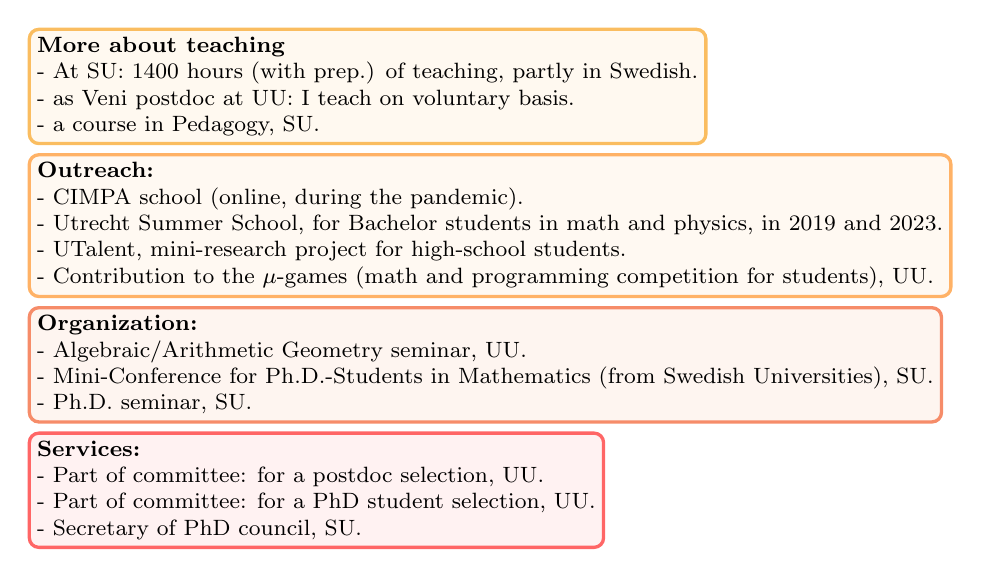
\begin{tikzpicture}
          [
          objective/.style = {fill = white},
          more_teaching/.style={rectangle, rounded corners=1ex, draw=YellowOrange!60, fill=YellowOrange!5, very thick, minimum size=5mm},
          outreach/.style={rectangle, rounded corners=1ex, draw=orange!60, fill=orange!5, very thick, minimum size=5mm}, 
          org/.style={rectangle, rounded corners=1ex, draw=RedOrange!60, fill=RedOrange!5, very thick, minimum size=5mm}, 
          serv/.style={rectangle, rounded corners=1ex, draw=red!60, fill=red!5, very thick, minimum size=5mm}, 
          ]
          {\footnotesize
          \onslide<2->{
               \node[more_teaching] (more_teaching) at (0,0) {
                         \pbox{\textwidth}{ 
                              {\bf More about teaching}\\
                              - At SU: 1400 hours (with prep.) of teaching, partly in Swedish.\\
                              - as Veni postdoc at UU: I teach on voluntary basis.\\
                              - a course in Pedagogy, SU.
                         }
                    };
          }
          \onslide<3->{
               \node[outreach, below=0.1cm of more_teaching.south west, anchor=north west ] (outreach) {
                         \pbox{\textwidth}{ 
                              {\bf Outreach:}\\
                              - CIMPA school (online, during the pandemic).\\
                              - Utrecht Summer School, for Bachelor students in math and physics, in 2019 and 2023.\\
                              - UTalent, mini-research project for high-school students.\\
                              - Contribution to the $\mu$-games (math and programming competition for students), UU.
                         }
                    };
          }
          \onslide<4->{
               \node[org, below=0.1cm of outreach.south west, anchor=north west ] (org) {
                         \pbox{\textwidth}{ 
                              {\bf Organization:}\\
                              - Algebraic/Arithmetic Geometry seminar, UU.\\
                              - Mini-Conference for Ph.D.-Students in Mathematics (from Swedish Universities), SU.\\
                              - Ph.D. seminar, SU.
                         }
                    };
          }
          \onslide<5->{
               \node[serv, below=0.1cm of org.south west, anchor=north west ] (serv) {
                         \pbox{\textwidth}{ 
                              {\bf Services:}\\
                              - Part of committee: for a postdoc selection, UU.\\
                              - Part of committee: for a PhD student selection, UU.\\
                              - Secretary of PhD council, SU.
                         }
                    };
          }
          }
	  \end{tikzpicture}  
\end{frame}

\begin{frame}{Teaching and supervision proposals in Nice}
     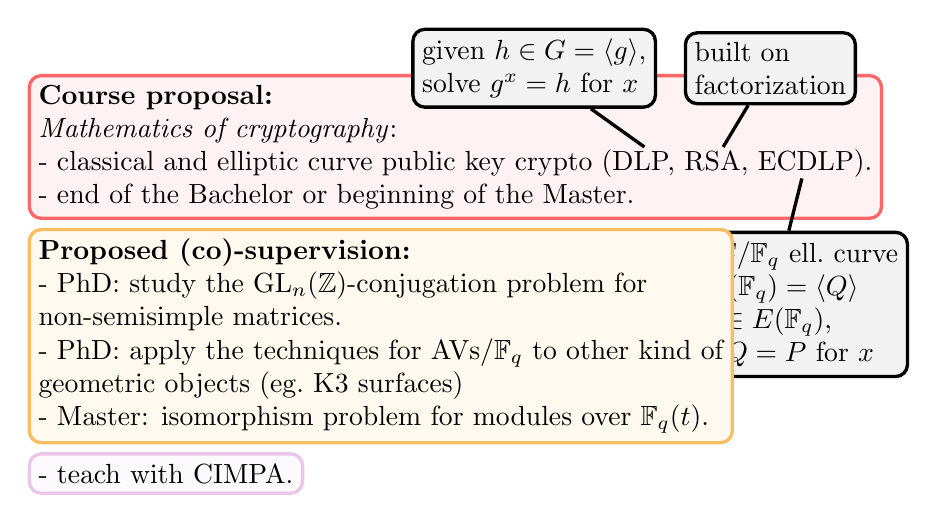
\begin{tikzpicture}
          [
          objective/.style = {fill = white},
          teaching/.style={rectangle, rounded corners=1ex, draw=red!60, fill=red!5, very thick, minimum size=5mm},
          blob/.style={rectangle, rounded corners=1ex, draw=Black!100, fill=Black!5, very thick, minimum size=5mm},
          superv/.style={rectangle, rounded corners=1ex, draw=YellowOrange!60, fill=YellowOrange!5, very thick, minimum size=5mm},
          cimpa/.style={rectangle, rounded corners=1ex, draw=Plum!60, fill=Plum!5, very thick, minimum size=5mm},
          ]
          \onslide<2->{
               \node[teaching] (teaching) at (0,0) {
                         \pbox{\textwidth}{
                              {\bf Course proposal:}\\
                              \emph{Mathematics of cryptography}:\\ 
                              - classical and elliptic curve public key crypto (DLP, RSA, ECDLP).\\
                              - end of the Bachelor or beginning of the Master.
                         }
                    };
          }
          \onslide+<3-5>{
               \node[blob] (blob1) at (1,1) {
                         \pbox{\textwidth}{
                              given $h \in G=\langle g \rangle$,\\
                              solve $g^x=h$ for $x$
                         }
               };
               \draw[-,draw=Black,very thick] (2.4,0) to (blob1); 
          }
          \onslide+<4-5>{           
               \node[blob] (blob2) at (4,1) {
                    \pbox{\textwidth}{
                         built on\\
                         factorization
                    }
               };
               \draw[-,draw=Black,very thick] (3.4,0) to (blob2);   
          }
          \onslide+<5>{
               \node[blob] (blob3) at (4,-2) {
                    \pbox{\textwidth}{
                         given $E/\F_q$ ell.~curve\\
                         with $E(\F_q) = \langle Q \rangle$\\
                         and $P \in E(\F_q)$,\\
                         solve $xQ=P$ for $x$
                    }
               };
               \draw[-,draw=Black,very thick] (4.4,-0.4) to (blob3); 
          }     
          \onslide<6->{
               \node[superv, below=0.1cm of teaching.south west, anchor=north west ] (superv) {
                         \pbox{\textwidth}{
                              {\bf Proposed (co)-supervision:}\\
                              - PhD: study the $\GL_n(\Z)$-conjugation problem for\\
                              non-semisimple matrices.\\
                              - PhD: apply the techniques for AVs/$\F_q$ to other kind of\\
                                geometric objects (eg.~K3 surfaces)\\
                              - Master: isomorphism problem for modules over $\F_q(t)$.
                         }
                    };
          }
          \onslide<7->{
               \node[cimpa, below=0.1cm of superv.south west, anchor=north west ] (cimpa) {
                         \pbox{\textwidth}{
                              - teach with CIMPA.
                              }
                    };
          }
	  \end{tikzpicture}  
\end{frame}

\begin{frame}{ }
My \textcolor{blue}{qualities}:
\begin{itemize}
     \item Variety of research themes \textcolor{gray}{(arithmetic, integral matrices, comm.~alg.)}.
     \item Computational expertise. \textcolor{gray}{(Magma)}.
     \item International profile. \textcolor{gray}{(IT $\to$ NL $\to$ SE $\to$ DE $\to$ NL $\to$ ?)}.
     \item International collaborations. \textcolor{gray}{(MIT, UU, SU, LU, HI, IMB)}.
     \item Grant writing skills. \textcolor{gray}{(Veni, K\&A W)}.
     \item Passion for teaching and pedagogical skills. \textcolor{gray}{(CIMPA, supervision, ... )}.
\end{itemize}
\vspace{1em}
\pause
My \textcolor{red}{integration} in Nice:
\begin{itemize}
     \item Branch out towards arithmetic.
     \item Strengthen current research themes \textcolor{gray}{(singularities)}.
\end{itemize}
\vspace{1em}
\pause
\begin{center}
% { \Large Thank you for your attention! }
{\Large Merci de votre attention!}
\end{center}
\end{frame}

\end{document}
